\documentclass[11pt,a4paper,fleqn,usenatbib,twocolumn]{mnras}

% MNRAS is set in Times font. If you don't have this installed (most LaTeX
% installations will be fine) or prefer the old Computer Modern fonts, comment
% out the following line
\usepackage{newtxtext,newtxmath}

% Depending on your LaTeX fonts installation, you might get better results with one of these:
%\usepackage{mathptmx}
%\usepackage{txfonts}

%\hypersetup{draft}
\usepackage{hyperref}
\usepackage{ulem}
\renewcommand{\ULdepth}{4pt}

% Use vector fonts, so it zooms properly in on-screen viewing software
% Don't change these lines unless you know what you are doing
\usepackage[T1]{fontenc}
\usepackage{ae,aecompl}

% Only include extra packages if you really need them. Common packages are:
\usepackage{graphicx}	% Including figure files
\usepackage{amsmath}	% Advanced maths commands
%\usepackage{amssymb}	% Extra maths symbols

%%%%%%%%%%%%%%%%%%% TITLE PAGE %%%%%%%%%%%%%%%%%%%

\title[Chemical enrichment]{Chemical enrichment}
\author[Camila A. Correa]{}

% These dates will be filled out by the publisher
%\date{Accepted XXX. Received YYY; in original form ZZZ}

% Enter the current year, for the copyright statements etc.
%\pubyear{2015}

% Don't change these lines
\begin{document}

%\maketitle

\section{Chemical enrichment}

We consider three different channels that contribute to the metal enrichment: Type Ia Supernovae (SNIa), core-collapse supernovae (CC-SNe) and asymptotic giant branch stars (AGB). For CC-SNe and AGB, the metal enrichment is mass and metallicity dependent, i.e. the elemental enrichment and the remnant mass depend on stellar metallicity as well as the mass of dying stars. SNIa, on the other hand, follow a different explosion path and we do not consider a metallicity dependence. 

To calculate the stellar mass fraction by chemical species that is returned to the ISM in a Hubble time, per stellar mass formed, at solar metallicity, we extract from the yield tables the mass, $M_{k}(M_{i},Z)$ (of a given element $k$), that is ejected into the ISM by a star (with initial mass $M_{i}$, and metallicity $Z$) over its lifetime. We integrate $M_{k}(M_{i},Z)$ over the Chabrier (2003) IMF $\phi(M)$ and normalize by the integral of the star masses over the IMF. Specifically, the return stellar mass fraction, $f_{k}$, of element $k$, is calculated as follows

\begin{equation}
f_{k} = \frac{\int_{{\rm{min}}(M_{Z}(t<t_{H}))}^{100~{\rm{M}}_{\odot}}  \phi(M_{i})\times M_{k}(M_{i},Z) {\rm{d}}M_{i}}{\int_{0.1~{\rm{M}}_{\odot}}^{100~{\rm{M}}_{\odot}} \phi(M_{i})\times M_{i}{\rm{d}}M_{i}}
\end{equation}

\noindent where the numerator corresponds to the total mass ejected of element $k$ per unit volume by stars with lifetimes shorter than a Hubble time ($M_{Z}(t<t_{H})$), and the denominator corresponds to the total stellar mass formed per unit volume. To calculate the star lifetimes we follow Wiersma et al. (2009) and use the inverse of the lifetime function from Portinari et al. (1998).

The stellar mass that is returned to the ISM by Type Ia supernovae depends on the number of SNIa events per unit stellar mass over a Hubble time,

\begin{equation}
N_{\rm{SNIa}} = \nu\left(e^{-t_{\rm{min}}/\tau}-e^{-t_{H}/\tau}\right),
\end{equation}

\noindent where $\nu=2\times 10^{-3}~\rm{M}_{\odot}^{-1}$, $t_{\rm{min}}$=40 Myr, $\tau=$2 Gyr, and $t_{H}$ is the Hubble time. The stellar mass fraction ejected into the ISM by SNIa is calculated as follows

\begin{equation}
f_{k} = \frac{\int_{{\rm{min}}(M_{Z}(t<t_{H}))}^{100~{\rm{M}}_{\odot}}  \phi(M_{i})\times N_{\rm{SNIa}}\times M_{i}\times M_{k} {\rm{d}}M_{i}}{\int_{0.1~{\rm{M}}_{\odot}}^{100~{\rm{M}}_{\odot}} \phi(M_{i})\times M_{i}{\rm{d}}M_{i}}.
\end{equation}

\begin{table*}
\begin{center}
\begin{tabular}{l|l|l|l}
\hline
& EAGLE & TNG & Illustris\\
\hline
AGB & Marigo (2001) & Karakas (2010) & Karakas (2010) \\
& [0.85-5]M$_{\odot}$, $Z{\in}$[0.004, & [1-6]M$_{\odot}$, $Z{\in}$[0.0001, 0.004, & [1-6]M$_{\odot}$, $Z{\in}$[0.0001, 0.004, \\
& 0.008, 0.02] & 0.008, 0.02] & 0.008, 0.02]\\
&  & Doherty et al. (2014)  &\\
&  & [7.0,7.5]M$_{\odot}$, $Z{\in}$ [0.004, 0.008, 0.02]&\\
&  & Fishlock et al. (2014) & \\
&  & [7.0]M$_{\odot}$, $Z{\in}$ [0.001] &\\\\
SNIa & Thielemann et al. (2003) & Nomoto et al. (1997) & Thielemann et al. (2003)\\
& & & Travaglio et al. (2004)\\\\
SNII &  Portinari et al. (1998) & Kobayashi et al. (2006) & Portinari et al. (1998) \\
& [6-120]M$_{\odot}$, $Z{\in}$ [0.0004, & [13-40]M$_{\odot}$, $Z{\in}$ [0,0.001, 0.004, 0.02] & [6-120]M$_{\odot}$, $Z{\in}$ [0.0004, 0.004,\\
& 0.004, 0.008, 0.02, 0.05] & Portinari et al. (1998) & 0.008, 0.02, 0.05]  \\
& & [6-13,40-120]M$_{\odot}$, $Z{\in}$ [0.0004, 0.004, \\
& & 0.008, 0.02, 0.05]\\
\hline
\end{tabular}
\end{center}
\caption{Overview of the stellar yield tables adopted in the EAGLE, TNG and Illustris galaxy formation models.}
\label{YieldTables}
\end{table*}

\begin{figure} 
\begin{center}
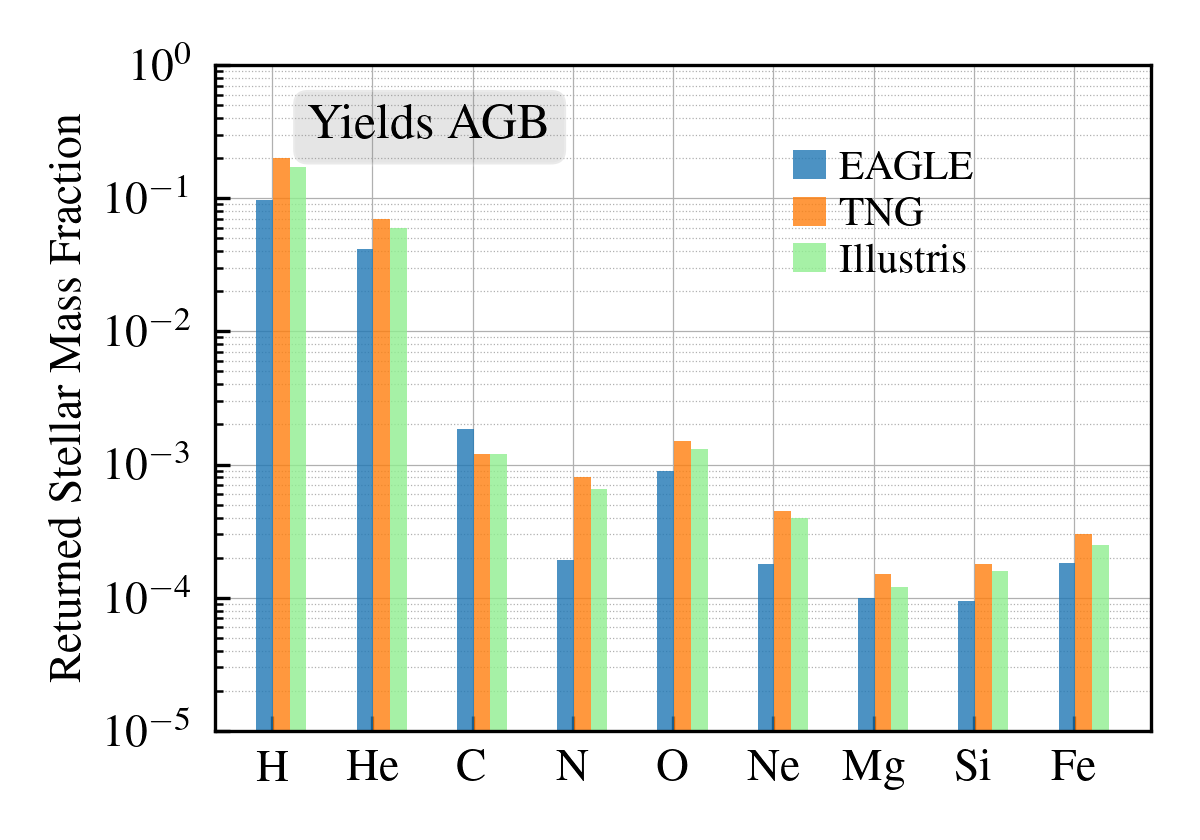
\includegraphics[angle=0,width=0.5\textwidth]{../figures/Comparison_AGBYield_tables_NoCOLIBRE.png}\\
\caption{Fraction of mass returned to the ISM in a Hubble time per stellar mas formed at Solar metallicity. The figure compares the mass returned by AGB enrichment from the EAGLE, TNG and Illustris galaxy formation model.}
\label{AGByields}
\end{center}
\end{figure}

\begin{figure} 
\begin{center}
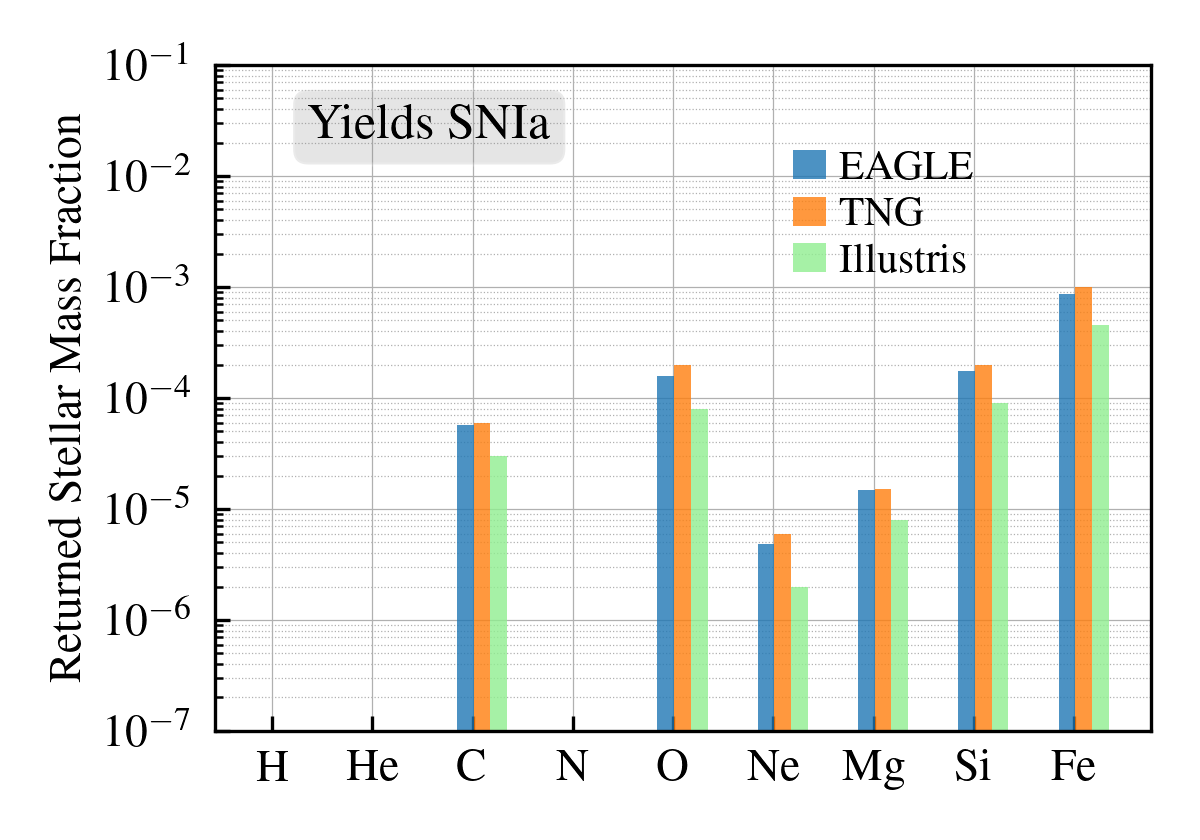
\includegraphics[angle=0,width=0.5\textwidth]{../figures/Comparison_SNIaYield_tables_NoCOLIBRE.png}\\
\caption{Fraction of mass returned to the ISM in a Hubble time per stellar mas formed at Solar metallicity. The figure compares the mass returned by SNIa enrichment from TNG, Illustris and EAGLE models.}
\label{SNIayields}
\end{center}
\end{figure}

\begin{figure} 
\begin{center}
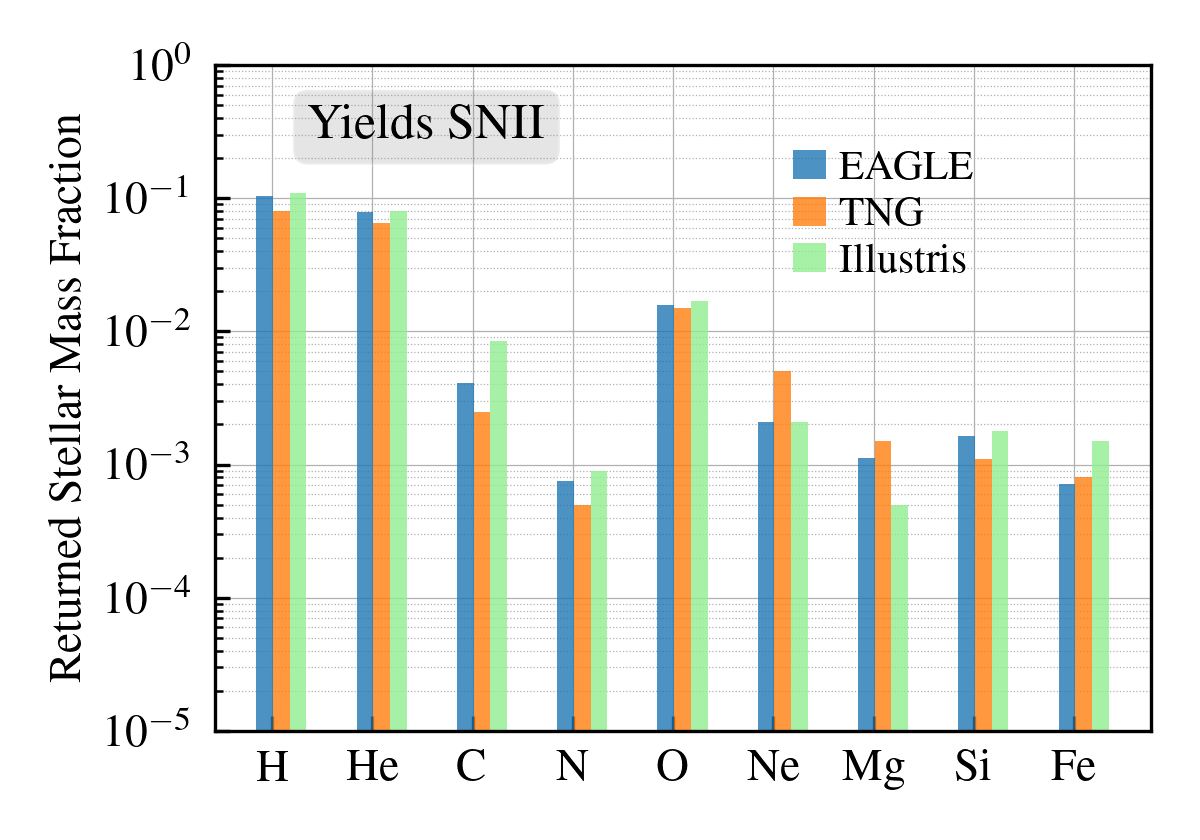
\includegraphics[angle=0,width=0.5\textwidth]{../figures/Comparison_SNIIYield_tables_NoCOLIBRE.png}\\
\caption{Fraction of mass returned to the ISM in a Hubble time per stellar mas formed at Solar metallicity. The figure compares the mass returned by SNII enrichment from the EAGLE, TNG and Illustris galaxy formation model. Note that EAGLE and Illustris adopt the same yield tables for SNII (see table), but EAGLE employs additional boost factors to boost (or decrease) the yields of some elements (see Wiersma et al. 2009, for further details).}
\label{SNIIyields}
\end{center}
\end{figure}



%\bibliography{biblio}
%\bibliographystyle{mnras}

\end{document}